
\documentclass{article}

\usepackage{amssymb,amsmath}
\usepackage{graphicx}
\usepackage{floatflt}
\usepackage[left=1in,top=1in,right=1in]{geometry}
\usepackage{hyperref}

\hypersetup{
    bookmarks=true,         % show bookmarks bar?
    unicode=false,          % non-Latin characters in Acrobat�s bookmarks
    pdfborder={0 0 0 0},
    pdfnewwindow=true,
    pdftoolbar=true,        % show Acrobat�s toolbar?
    pdfmenubar=true,        % show Acrobat�s menu?
    pdffitwindow=true,      % page fit to window when opened
    pdftitle={System Requirements Specification},    % title
    pdfauthor={Andrew Atutis, Joe Belmont, Steve Deyo, Ryan Edgar, Jon Eggleston, John Ellis, Jacor Finlayson, Michael Hadley, James Licata, Brett Peplowski},     % author
    pdfsubject={EE418: Software Engineering Senior Design},   % subject of the document
    pdfkeywords={keywords}, % list of keywords
    colorlinks=false       % false: boxed links; true: colored links
}

\usepackage{xr}
\externaldocument{high_level_design}


\title{Activity Monitor}
\author{Andrew Atutis \and Joe Belmont \and Steve Deyo \and Ryan Edgar \and Jon Eggleston \and John Ellis \and Jacor Finlayson \and Michael Hadley \and James Licata \and Brett Peplowski}
\date{\today}


\setcounter{tocdepth}{3}

\begin{document}

\begin{titlepage}
\maketitle
\end{titlepage}


\tableofcontents

\newpage

\section{Introduction}

\subsection{Purpose}
The system will provide a better way to monitor Patient rehabilitation.  The system will be targeted towards nursing homes and rehab hospitals which require monitoring of elderly people, recovering athetes, and people with balance issues. The system will further provide independent mobility while monitoring a Patients progress.

\subsection{Project Scope}
To develop a mobile pedemeter, that is worn by the Patient. The device must be cheap, wireless, rugged and easy to use. Build a system to monitor activity inside and outside the home. The device can be used as a monitoring tool for compliance with perscribed activities intended for theraputic development of motor functions.

\subsection{Business Context}
The requirements of the project are drawn from the anticipated needs of Patients, Clinicians, and researches working in rehabilitation hospitals and nursing homes.  Limited funding will be provided by the Software Engineering Department at Clarkson University. The timeline indicates the project must be completed in a 15 week period.  Each member of the team is also a full time student and therefore has a constrainted amount of time and effort to be put forth relative to a full time employee.

\subsection{Definitions}\label{defs}

\begin{itemize}
\item Clinician - Person directing and monitoring Patients, their progress, and their daily tasks.

\item Researcher - Person interested in analyzing data collected by the system to find trends to help Clinicians in diagnosis and therapy.

\item Administrator - Power user whose main job is to Add/Remote/Edit Researchers and Clinician accounts for the Web UI.

\item PDA - Personal Digital Assistant, device the Patient carries that records and interfaces with Wii Remote.

\item Wii Remote - Item worn by Patient to help record information during a Daily Task, a controller component familiar to the Nintendo Wii system.

\item Bluetooth - Open wireless protocol for exchanging data over short distances from fixed and mobile devices, used between Wii Remote and PDA.

\item Web UI (to be named later) - Interface used by Clinician's and Researcher's to access and edit Patient information.

\item Patient Profile - Area accessed and maintained by Clinicians via the Web UI, where Patient data and progress are represented.
			The following data is provided about the Patient: Full Name, Patient Number, DOB, Height, Weight, Gender, Address, Phone
			Email (optional), Social Security Number, Username, Password, and Medical Conditions. 

\item Clinician Profile - Area accessed by Clinicians after logging into the Web UI, where Patient list and Clinician information are represented.

\item Clinician Account - The account for a specific Clinician on the Web UI. Contains the following information: Full Name, Clinician Number, Address, Phone, List of Patients assigned to this Clinician, Username, Password

\item Clinician Charts - This includes two charts that the Clinician can use to monitor a specific Patient's progress: Patient Health Charts and Patient Completion Charts. Each of these charts will represent an individual Patient, and a Clinician can only view these charts for Patients registered to him/her.

\item Researcher Profile - Area accessed by Researchers after logging into the Web UI, where data from Patients can be represented collectively for analysis.

\item Researcher Account - The account for a specific Researcher on the Web UI. Contains the following information: Full Name, Researcher Number, Address, Phone, Username, Password

\item Researcher Charts - This includes three charts that the Researcher can view to collect Patient information: Patient Health Charts, Group Patient Charts, and Patient Completion Charts. Two of these charts are identical to the Clinician Charts (Patient Health Chart and Patient Completion Chart) however, the Patient names will be anonymous. 

\item Server - Windows Server box running in remote location, where the PDA sends its data to be stored in the database. Also accessed by the Web UI to obtain database information for the Web UI.

\item Client GUI - Interface used by the Patients on the PDA. Allows user to view tasks, current progress, and statistics about their current daily task.

\item Daily Task - Exercise and instructions ordered to a Patient by a Clinician.  This is generally the number of steps that must be walked in a day.

\item Data Dump - When the PDA sends its recorded Patient information to the Server.

\item PDA Statistics Page - A section of the PDA front-end GUI application that displays computed PDA Statistics from Daily Tasks for the past week. 

\item PDA Statistics - Numeric quantities calculated from the raw Wii Remote data: Steps Taken, Distance, Calories Burned, Steps per Minute, Time Walking and Average Speed.  
\end{itemize}

\section{Overall Description}

\subsection{Product Functionality}	
The system will provide the following features:
\begin{enumerate}
\item The Wii Remote attached to the Patient's belt will transmit walking data to the PDA carried by the Patient.
\item The PDA will transmit data to a remote server as well as update the Patient's tasks periodically. 
\item A Web UI will be hosted by the server that allows Clinicians/Researchers to login to view Patient progress, statistics, chart/graph trends, etc. 
\item A PDA UI that will be running in Windows Mobile that will interface with the Wii Remote. This UI will also provide Patients with "Tasks for the Day" as well as a "PDA Statistics Page".
\end{enumerate}

\subsection{System Context}
This system is comparable to an everyday pedometer used to monitor walking activity. The major improvement lies in the interactive features provided to the Clinician Researcher and Patient. Real-time data analysis and feedback is provided to help ensure effective Patient treatment. This system provides the ability to have both independent mobility as well as closely monitored workout regimens. 

\subsection{User Characteristics}

\subsubsection{Administrator}
This user's main concern is to manage Clinician and Researcher accounts on the Web UI. They will be responsible for Adding/Removing/Editing these accounts.

\subsubsection{Clinician}
This user's main concern will be view the progress of a particular Patient on a particular set of tasks. This user only wants to view information about a specific Patient. From this information the Clinician can manage the Patient's Daily Tasks. No computing knowledge is assumed, the Web UI will be learned in 1 to 2 hours. 

\subsubsection{Researcher}
This user's main task will be to view and identify useful trends in the database. The Researcher will work side-by-side with the Clinician in order to improve Daily Task regimens. This user will focus their efforts on Patients as a whole, and how they are performing against these Daily Task regimens. No computing knowledge is assumed, the Web UI will be learned in 1 to 2 hours.

\subsubsection{Patient}
This user is only concerned with rectifying their personal wellness. There are some underlying assumptions made about the Patient/caregiver for use of this system:
\begin{enumerate}
\item Some amount of manual dexterity (interact with the PDA touch-screen)
\item Clear vision (can observe walking statistics, read alert messages, etc.)
\item Ability to read written English words on the PDA
\item Good hearing (can react to PDA alerts)
\end{enumerate}
No assumptions are made about the level of PC literacy of the Patient/caregiver.


\subsection {Operation Environment}

\begin{enumerate}
\item PDA - Palm Treo 750 running Windows Mobile 5
\item Remote server running Windows Server
\end{enumerate}

The PDA and Wii Remote will be carried by the Patient when a Daily Task is performed. The Server will be located in a remote location (at the rehab hospital, clinic, etc.). The Clinician and Researcher will log onto the Web UI hosted by the server via a remote machine.

\subsection {Design and Implementation Constraints}

\begin{enumerate}

\item Limited Budget - Limited funds constricts our options concerning both hardware and software. This may prevent us from using the best and most efficient tools that would better the project.

\item Limited Time - All developers are full-time students who need to dedicate their time to other assignments and projects as well.

\item Licensing Issues - Both the PDA and Wii Remote were developed by outside parties. This may bring up lisencing issues concerning what we want to use the products for and how we want to use them, as opposed to what the developer companies allow them to be used for.

\item PDA use is restricted to using only the Palm Treo. A Windows OS is required for the PDA/server implementation.

\item GUI's must be developed as easy to use for non-technologically savvy individuals, including the elderly and young children.

\end{enumerate}


\subsection {User Objectives}

The Clinician wants to view the progress of a particular Patient and provide feedback to that Patient regarding their performance. The Clinician will achieve this through statistics/charts/graphs displayed in the Web UI. 
The Researcher wants to identify useful trends present in groups of Patient data. The Researcher will achieve this through statistics/charts/graphs displayed in the Web UI. 
The Patient wants to improve their personal wellness. The system will help the Patient achieve this by:
\begin{enumerate}
\item Providing real-time feedback/statistics to the Patient whilst exercising
\item Provide statistics for the past week
\item Providing an easy to use interface that shows the specific tasks for the day
\end{enumerate}

\subsection {Assumptions}
\begin{enumerate}
\item The PDA is able to make a secure, reliable Bluetooth connection to the PDA and successfully transfer raw data from the Wii Remote to the PDA.
\item The PDA has enough room to store a days worth of raw data from the Wii Remote.
\item The Wii Remote's battery life will last an entire day.
\item The PDA can connect to the server and pass transfer raw data and receive update information from server through a secure, reliable and wireless connection.
\item The PDA can run scripts that process raw data from Wii Remote.
\item The raw data received from Wii Remote is valid enough for calculating PDA Statistics (see "PDA Statistics" in Definitions, Section \ref{defs}).
\item The Patient is savvy enough to understand that both the PDA and Wii Remote must be on and connected in order to begin recording their progress for the day.
\item Clinicians and Researches have internet access and are savvy enough to navigate through a UI that requires a secure login and other navigation.
\end {enumerate}


\section{System Features}

\subsection{High Priority}

\subsubsection{Application Start and Statistics Display}\label{sec: App Start}

\paragraph{Description}
The Patient starts the application and is brought immediately into their account with the PDA Statistics Page showing. In the background, the PDA begins recording data towards the Daily Task.

\paragraph{Stimulus/Response}
The user starts the client application, the application starts and they are brought to the statistics page. All of the PDA Statistics
are displayed from the last Daily Task (see "PDA Statistics" in Definitions, Section \ref{defs})

\paragraph{Functional Requirements}
\begin{enumerate}
\item The PDA is running the client application.  The Wii Remote is connected via Bluetooth to the PDA.  The PDA is able to get the data from the Wii Remote and turn it into useful data.
\item If the application fails to start correctly it will give an error message and exit.
\end{enumerate}

\paragraph{Test Plan}
\begin{enumerate}
\item The Patient starts up the client application successfully.  They are brought to the statistics page.
\item The Patient attempts to start up the client application but it fails.  They are shown an error message and then the application exits.
\end{enumerate}

\subsubsection{Data Dump}\label{sec: Data Dump}

\paragraph{Description}
The PDA sends the PDA Statistics it has collected to the server.  If the connection fails, the PDA will retry 10 times over the course of 10hrs. If after 10 times a connection cannot be established, the PDA will stop trying to connect for the day.
This Data Dump will be triggered at the end of a Patient's Daily Task.

\paragraph{Stimulus/Response}
The Patient has finished a Daily Task. An alert will be displayed on the PDA and the PDA will attempt to send the accumulated PDA Statistics to the server.

\paragraph{Functional Requirements}
\begin{enumerate}
\item The Wii Remote is connected via Bluetooth to the PDA. The PDA client is running and is collecting the data from the Wii Remote.  The server is running and is able to receive data from the PDA.
\item If the PDA fails to get a connection with the server it will stop trying for the day.
\end{enumerate}

\paragraph{Testplan}
\begin{enumerate}
\item The test begins with the Wii Remote sending data to the PDA.  Once the PDA has collected the data for the day, it successfully dumps the data to the server.
\item The test begins with the Wii Remote sending data to the PDA.  Once the PDA has collected the data for the day, it attempt to send the data to the server but fails.  The PDA will keep trying to send data to the server.
\end{enumerate}


\subsubsection{Emergency Data Dump}\label{sec: Emer Data Dump}

\paragraph{Description}
The PDA has used more than 95\% of the memory allocated to data storage. The PDA will then attempt to connect to the server and the dump its current PDA Statistics to the server.

\paragraph{Stimulus/Response}
The PDA has failed doing a data dump on its normal interval.  The phone will keep trying to do a emergency data dump until the data is successfully received by the server, or the limit of 10 connection attempts has been exceeded over the 10hr period. Upon reaching this limit, the PDA will delete 10\% of the stored data, and make a note in the data log indicating the time period over which the data was deleted.

\paragraph{Functional Requirements}
\begin{enumerate}
\item The Wii Remote is connected via Bluetooth to the PDA.
\item The PDA client is running and is collecting the data from the Wii Remote. 
\item The server is running and is able to receive data from the PDA.
\item If the PDA keeps failing to get a connection with the server it will stay in Emergency Data Dump mode.
\item If 10 data dumps fail the PDA will delete 10\% of the stored data in order to keep recording.  A log entry will be inserted into the data log indicating over which period of time the data was deleted. The PDA will then display an error message about the failure to dump data on the PDA.
\end{enumerate}

\paragraph{Testplan}
\begin{enumerate}
\item The test begins with the PDA put into Emergency Data Dump mode.  The PDA will then dump the data to the server and exit Emergency Data Dump mode.
\item The test begins with the PDA put into Emergency Data Dump mode.  The PDA tries to dump data to the server but will fail.  The PDA will stay in Emergency Data Dump mode.
\item If the PDA fails connecting to the server 10 times it will erase 10\% of the data in memory in order to keep recording data.  The PDA will display an error message about the data dump and will instruct the user to call the Clinician and report the error.
\end{enumerate}



\subsubsection {Patient Profile}\label{sec: Patient Profile}
\paragraph {Description}
After the Clinician has logged into the web site hosted by the server, the Clinician will have the ability to create a profile for one of their Patients. This profile will contain all of the relevant Patient Profile information (see "Patient Profile" in Defintions, Section \ref{defs}) This profile will ultimately be linked to a specific PDA and also be associated with a certain prescribed exercise regiment. The information that is able to be displayed must be in compliance with the Health Insurance Portability and Accountability Act of 1996 (HIPA). In other words, must be properly protected while allowing the flow of health information needed to provide and promote high quality health care and to protect the public's health and well being.

\paragraph {Stimulus/Response}
The Clinician will navigate to the "Add Patient" page from their home page. A form will be presented that includes field for personal Patient data. The Clinician will complete form and will click the "Add Patient" button. The Clinician will be redirected toward their home page with a "Patient Successfully Added" message at the top.

\paragraph {Functional Requirements}
\begin{enumerate}
\item A web user interface needs to be implemented on the server which will allow the Clinician to log in and view their home page.
\item A navigation path must be present in order for the Clinician to access the "Add Patient" page from their home page. 
\item A form must be generated when the Clinician navigates to the "Add Patient" page. This form must including fields all relevant Patient Profile information (see "Patient Profile" in Defintions, Section \ref{defs}).
\item The Clinician must be able to complete the form and have all of the Patient data stored in the back-end database. 
\item The Clinician must be redirected to their home page. 
\item All information showed must be in compliance with the HIPA.
\end{enumerate}

If the Clinician leaves any fields empty, or enters an invalid value for any of the fields (except email), then the Clinician
will be redirected back to the "Add Patient" page with an error message as well as the incorrect fields highlighted in red.  

\paragraph {Test Plan}
\begin{enumerate}
\item Begins with the tester at the Clinician Home Page. The tester clicks on the "Add Patient" button. The tester is redirected to the "Add Patient" page where fields are presented for all relevant Patient Profile information (see "Patient Profile" in Defintions, Section \ref{defs}). The tester fills out all of the fields and clicks the "Add Patient" button. The tester is redirected to the Clinician Home Page with a message: "Patient successfully added".
\item Begins with the tester at the Clinician Home Page. The tester clicks on the "Add Patient" button and is redirected to the "Add Patient" page. The tester is presented with the proper fields. The tester enters non-alphabetic characters for the Name, or leaves one or more required fields blank. The tester completes the form by clicking the "Add Patient" button. The Clinician is redirected to the "Add Patient" page with a message: "Invalid input in one or more fields". The Name field is highlighted in red, as well as the fields that were previously left blank.
\end{enumerate}


\subsubsection {Web UI}\label{sec: Web UI}
\paragraph {Description}
Their must be a web user interface hosted by the server that provides a way for the Clinicians and Researchers to access data from the database in a useful way. This Web UI will be the primary tool used by Clinicians to monitor their Patients. This Web UI will be the primary tool used by Researchers to analyze trends in prescribed Daily Tasks.
\paragraph {Stimulus/Responses}
Raw Wii Remote Data as well as PDA Statistics (see "PDA Statistics" in Definitions, Section \ref{defs}) will be downloaded to the server periodically, which will be represented in the Web UI. Clinicians and Researchers will be able to query to database through this Web UI and receive the most recent statistics. 

\paragraph {Functional Requirements}
\begin{enumerate}
\item Provide a way to connect to the Web UI via a web browser on a remote machine.
\item Provide a secure connection that maintains the privacy of the Patients 	 
\item There must be a database connection so that the Web UI can display the most up-to-date statistics	
\item There must be software capabilities that allow for the transfer of data from the PDA to the server
\end{enumerate}

\paragraph {Test Plan}
\begin{enumerate}
\item The tester opens up a web browser on a remote machine. The tester points the web browser to the address of the server Web UI. The tester is presented with the user login page.
\item The tester is at the Clinician's Home Page. The tester adds a new Patient as specified by the "Add Patient" Test Plan 1. The tester views the new Patient on the Clinician Home Page as it was saved in the database. 
\item The tester logs into the Web UI as a Researcher right after a Patient has completed a Daily Task (all of the data has been downloaded to the server). The Researcher is able to view all of the updated Researcher Charts with the recently downloaded Daily Tasks from the PDA.  
\end{enumerate}

\subsubsection {Administrator can Add/Remove/Edit Researcher and Clinician Web UI Accounts} \label{sec: Administrator Add/Remote/Edit}
\paragraph {Description}
There must be an Administrator account that is initially active on the Web UI to allow for Add/Remote/Edit actions to be performed for Researcher and Clinician accounts.

\paragraph {Stimulus/Responses}
The Administrator will log onto the Web UI using a predetermined Username and Password. The Administrator's credentials are verified, and they are presented with the Administrator Homepage (see Feature \ref{sec: Administrator Homepage}).

\paragraph {Functional Requirements}
\begin{enumerate}
\item Provide a way to connect to the Web UI via a web browser on a remote machine.
\item Provide a secure connection that maintains the privacy of the Patients 
\item There must be an interface available that manages Researcher and Clinician accounts		 
\end{enumerate}

\paragraph {Test Plan}
\begin{enumerate}
\item The tester opens up a web browser on a remote machine. The tester points the web browser to the address of the server Web UI. The tester logs in as an Administrator. The tester is presented with the Administrator Homepage. From here, the tester clicks on the Add Researcher link. The tester is presented with a page to enter the Researcher's Account information (See "Researcher Account" in Definitions \ref{defs})
The tester presses the "Submit" button. The Researcher is added to the Database.
\item The tester opens up a web browser on a remote machine. The tester points the web browser to the address of the server Web UI. The tester logs in as an Administrator. The tester is presented with the Administrator Homepage. From here, the tester clicks on the Add Clinician link. The tester is presented with a page to enter the Clinician's Account information (See "Clinician Account" in Definitions \ref{defs})
The tester presses the "Submit" button. The Clinician is added to the Database.
\item The tester opens up a web browser on a remote machine. The tester points the web browser to the address of the server Web UI. The tester logs in as an Administrator. The tester is presented with the Administrator Homepage. From here, the tester clicks on the Remove Researcher link for a specific Researcher. The tester is prompted by a pop-up dialog to make sure that they a certain that they want to Remove this Researcher. The tester clicks "Yes" and the Researcher is removed from the Database. 
\item The tester opens up a web browser on a remote machine. The tester points the web browser to the address of the server Web UI. The tester logs in as an Administrator. The tester is presented with the Administrator Homepage. From here, the tester clicks on the Remove Clinician link for a specific Clinician. The tester is prompted by a pop-up dialog to make sure that they a certain that they want to Remove this Clinician. The tester clicks "Yes" and the Clinician is removed from the Database. 
\item The tester opens up a web browser on a remote machine. The tester points the web browser to the address of the server Web UI. The tester logs in as an Administrator. The tester is presented with the Administrator Homepage. From here, the tester clicks on the Edit Clinician link for a specific Clinician. The tester is presented with a page to edit the Clinician's Account information (See "Clinician Account" in Definitions \ref{defs})
The tester presses the "Submit" button. The changes to the Clinician's Account are added to the Database.
\item The tester opens up a web browser on a remote machine. The tester points the web browser to the address of the server Web UI. The tester logs in as an Administrator. The tester is presented with the Administrator Homepage. From here, the tester clicks on the Edit Researcher link for a specific Researcher. The tester is presented with a page to edit the Researcher's Account information (See "Researcher Account" in Definitions \ref{defs})
The tester presses the "Submit" button. The changes to the Researcher's Account are added to the Database.
\end{enumerate}

\subsubsection {Administrator Homepage} \label{sec: Administrator Homepage}
\paragraph {Description}
This Homepage is where the Administrator will be redirected to after Login. From here, the Administrator is presented with lists of Researchers and Clinicians who currently have accounts.
From here, the Administrator can click links to Add/Remove/Edit a specific Researcher or Clinician.
\paragraph {Stimulus/Responses}
The Administrator will log onto the Web UI using a predetermined Username and Password. The Administrator's credentials are verified, and they are presented with the Administrator Homepage.

\paragraph {Functional Requirements}
\begin{enumerate}
\item Provide a way to connect to the Web UI via a web browser on a remote machine.
\item Provide a secure connection that maintains the privacy of the Patients 
\item There must be an interface available that manages Researcher and Clinician accounts	 
\end{enumerate}

\paragraph {Test Plan}
\begin{enumerate}
\item The tester opens up a web browser on a remote machine. The tester points the web browser to the address of the server Web UI. The tester logs in as an 
Administrator. The tester is presented with the Administrator Homepage. 
\item The tester opens up a web browser on a remote machine. The tester points the web browser to the address of the server Web UI. The tester logs in as an 
Administrator. The Username and Password are rejected by the Server, and the tester is redirected to the Login screen. 
\end{enumerate}

\subsubsection{Unique Usernames for Clinicians and Patients}\label{sec: Unique Usernames}

\paragraph{Description}
Between the Web UI, PDA, and Database there must be a way to associate and organize users and their information. A Clinician must have a unique id from other Clinicians so that they can be assigned to certain Patients.
\paragraph{Stimulus/Response}
A Clinician will register on the Web UI to become a valid user to view a Patient Profile. The server must query the database to make sure that a Clinician does not make multiple accounts. 
The Clinician registers a new Patient by the Test Plan described in Feature 3.1.5 (Patient Profile). The "Username" field for the Patient Profile will be unique to each Patient. If a 
Username conflicts with another Patient, an error will be displayed on the "Add Patient" page. 
\paragraph{Functional Requirements}
\begin{enumerate}
\item Provide a way to register new Clinicians via the Web UI.
\item The Server must be able to detect and disallow duplicate Clinician Usernames.
\item The Server must be able to detect and disallow duplicate Patient Usernames when a Clinician creates a new Patient. 
\end{enumerate}

\paragraph{Test Plan}
\begin{enumerate}
\item The tester registers with the Web UI as a Clinician. The tester then successfully logs into the system and is able to add Patients via the "Add Patient" page
\item The tester registers with the Web UI as a Clinician. The tester is already registered with the system, and the Web UI alerts the tester that the Username is taken.
\item The tester adds a Patient using the Web UI via the "Add Patient" page. This Patient's Username is already registered with the system. The Web UI redirects the tester
back to the "Add Patient" page with an error message.
\end{enumerate}

\subsubsection {PDA to Wii Remote Connection}\label{sec: PDA Wii Conn}
\paragraph {Description}
This is priority high and this is to connect both compatible Bluetooth components from the Wii Remote and the PDA.  Once connection is established they are exclusively paired to each other.

\paragraph {Stimulus/Response}
Once connection is made an alert to the client from the PDA acknowledges pairing as well as a vibration from the Wii Remote for double assurance.

\paragraph {Functional Requirements}
\begin{enumerate}
\item Bluetooth components must be compatible to initially be in discoverable mode in order to pair.
\item If for any reason the connection is interrupted or lost, the text/audio alert use case is implemented to notify the client. 
\end{enumerate}

\paragraph {Test Plan}
\begin{enumerate}
\item Begin with the tester on the PDA establishing it in discoverable mode. Then proceed to turn on the Wii Remote to put it in discoverable mode as well.  At that point after each device finds the other, the tester approves the connection of the PDA and the Wii Remote and PDA enter the paired mode. 
\item Begin with the tester on the PDA establishing it in discoverable mode. Then proceed to turn on the Wii Remote to put it in discoverable mode as well. If the devices are not within the Bluetooth range then the PDA will prompt that the device has not been found and at that point  both the Wii Remote and PDA must be brought closer in order to be within scope of the Bluetooth component.
\end{enumerate}

\subsubsection {PDA to Server Connection}\label{sec: PDA Server Conn}
\paragraph {Description}
This is priority high and is the connection that must be instituted from the PDA to the Server in order to send PDA Statistics from the Patient's Daily Tasks. 
 
\paragraph {Stimulus/Response}
The Clinician will set up the Patient accound on the PDA via the Clinician GUI. The Clinician will pair the Wii Remote and the PDA as well. 

 
\paragraph {Functional Requirements}
\begin{enumerate}
\item If connection between the PDA and the server is lost then frequent attempt to reconnect is commenced.
\item More in particular it will be on a given interval that reconnection attempts are made and the use case of connection-loss detection is started.
\end{enumerate}


\paragraph {Test Plan}
\begin{enumerate}
\item Begins with the tester on the PDA and a connection attempt is made to the server.  If connection is successful, mock data is sent to the server for assurance.
\item Begins with the tester on the PDA and a connection attempt is made to the server.  If connection is ineffective, the PDA will alert unsuccessful for the connection.  From there the PDA will automatically make reconnection attempts on a certain interval time until connection is made. 
\end{enumerate}

\subsubsection {Clinician GUI for Initial Patient Login on the PDA}\label{sec: Clinician GUI}
\paragraph {Description}
This is a high priority feature that gives the Clinician the ability to set up the Patient's account on the PDA. This GUI will be easy-to-use and will allow the Clinician to enter the Patient's unique Username/Password
combination as specified in the Server's Database. There will also be a button off to the side at the Patient's home page (on the PDA) that allows the Clinician to modify the Patient's login info.
 
\paragraph {Stimulus/Response}
The Clinician will be presented with the page that asks him/her to enter the Patient's Username and Password. Once the Clinician enters the correct credentials for a specific Patient, the PDA is then paired to the Wii Remote. 
If the wrong credentials are entered, the Clinician will be prompted until he/she enters the proper Username and Password. Once the PDA and Wii Remote are paired, the Patient will not have to login when they start up the Activity Monitor Application.

\paragraph {Functional Requirements}
\begin{enumerate}
\item The Username and Password for a particular Patient must be stored locally on the PDA. 
\item There must be a unique Username/Password combination for each Patient.
\end{enumerate}

\paragraph {Test Plan}
\begin{enumerate}
\item Begins with the tester attempting to start the Activity Monitor application. This is the first time the PDA has started this application. The application will display the Clinician Login page asking fot the Patient's Username and Password. The proper Username and Password are entered, and the PDA is then paired with the Wii Remote.
\item Begins with the tester attempting to start the Activity Monitor application. This is the first time the PDA has started this application. The application displays the Clinician Login page. The Clinician enters the wrong Username and Password combination and is redirected back to the login page until the proper credentials are entered. 
\item The Patient starts the Activity Monitor application. The Patient is redirected right to the home page (not asked for Username and Password).
\end{enumerate}


\subsubsection {Connection mode: paired, discoverable}\label{sec: Conn Mode}
\paragraph {Description}
This is priority high; the Bluetooth components must have a discoverable mode in order for the Wii Remote and the PDA to sync, which in result should have a paired mode to recognize the connection between the two.

\paragraph {Stimulus/Responses}
A vibration and an alert are given when exiting discoverable mode and officially entering paired mode.

\paragraph {Functional Requirements}
\begin{enumerate}
\item Provide a way to connect to the Web UI via a web browser on a remote machine.
\item Provide a secure connection that maintains the privacy of the Patients 	 
\item There must be a database connection so that the web user interface can display the most up-to-date data/statistics	
\item There must be software capabilities that allow for the transfer of data from the PDA to the server
\end{enumerate}

\paragraph {Test Plan}
\begin{enumerate}
\item The tester has the Wii Remote and PDA, and attempts to put the Bluetooth components in discoverable mode. Once that is accomplished the tester uses the PDA and attempts to pair both devices. If successful, then both modes are supported. If not successful, then both modes aren't supported and an alert on the PDA acknowledges the tester.
\end{enumerate}

\subsubsection{PDA records data from Wii Remote}\label{sec: PDA Records Data}

\paragraph{Description}
The PDA will record the incoming Raw Wii Remote Data and summarize this data into PDA Statistics. The PDA will then delete the Raw Wii Remote Data after processing.

\paragraph{Stimulus/Response}
The Patient starts up the Activity Monitor Application on the PDA. The PDA sends a message to the Wii Remote indicating that it is ready to start receiving data. Data transfer begins through a Bluetooth connection. The PDA receives the Raw Wii Remote Data and processes it into PDA Statistics. The Raw Wii Remote Data is deleted from the PDA  to conserve space. 

\paragraph{Functional Requirements}
\begin{enumerate}
\item Both devices must be on and synched.
\item A wireless Bluetooth connection must be present to transfer the Raw Wii Remote Data to the PDA in a desired directory.
\item Data sampling must be used while recording data from the Wii Remote.
\item If connection between PDA and Wii Remote is lost during recording, the PDA must regularly attempt to automatically re-synch.
\item All pedometer functionality must be able to cope with intermittent data loss.
\end{enumerate}

\paragraph{Test plan}
\begin{enumerate}
\item The Patient has started their exercise for the day and the PDA automatically beings receiving and processing raw data from the Wii Remote, utilizing data sampling. The PDA Statistics are stored on the PDA.
\item The Patient has started their exercise for the day and the PDA automatically beings receiving and processing raw data from the Wii Remote, utilizing data sampling. The PDA Statistics are stored on the PDA. The connection between Wii Remote is lost, the PDA and Wii Remote automatically reconnect and begin transferring raw data automatically. All pedometer functionality and data graphs must be able to handle missing data case.
\item The Patient has started their exercise for the day and the PDA automatically beings receiving and processing raw data from the Wii Remote, utilizing data sampling. The PDA Statistics are stored on the PDA. The Patient has indicated they are done exercising for the day, data transfer stops.
\end{enumerate}


\subsubsection {Alerts on PDA Including Text and Audio}\label{sec: Alerts}
\paragraph{Description}
The PDA is able to report various situations to the Patient depending on the status of the Wii Remote. It can do this through both text alerts and audio alerts.

\paragraph {Stimulus/Response}
A situation arises in which the PDA is required to send a message to the Patient. It sends them an audio signal that makes them aware of the alert. Upon checking the PDA, the Patient will now see a text alert describing the situation to them with instructions on what to do next.

\paragraph {Functional Requirements}
\begin{enumerate}
\item Alerts must be sent when:
\item Connection between PDA and Wii Remote is connected, reconnected and interrupted
\item Connection is made/lost between the PDA and server
\item Battery of Wii Remote and/or PDA is low
\item Battery of Wii Remote is dead
\item A Daily Task is completed		 
\end{enumerate}

\paragraph {Test Plan}
\begin{enumerate}
\item Begin with the tester performing a Daily Task. The tester then turns off the Bluetooth functionality on the PDA. Once the interrupted connection between the Wii Remote and the PDA is detected, the PDA will emit a series of beeps. Upon checking the PDA, the tester should receive a text alert describing the interrupted connection with instructions on what to do next.
\item Begin with the tester performing a Daily Task. The tester then turns off the server. Once the interrupted connection between the PDA and the server is detected, the PDA will emit a series of beeps. Upon checking the PDA, the tester should receive a text alert describing the interrupted connection with instructions on what to do next. Once instructions are followed/situation is resolved, the alert message disappears.
\item Begin with the tester performing a Daily Task. The tester then turns off the server. Once the interrupted connection between the PDA and the server is detected, the PDA will emit a series of beeps. Upon checking the PDA, the tester should receive a text alert describing the interrupted connection with instructions on what to do next. Once instructions are followed/situation is resolved, the alert message disappears.
\item The tester waits for the battery on the Wii Remote to wear down.  As the battery in the Wii Remote becomes low, the PDA emits a series of beeps.  Upon checking the PDA, the tester should receive a text alert describing the low battery with instructions on what to do next. Once instructions are followed/situation is resolved, the alert message disappears.
\item The tester waits for the battery on the Wii Remote to die.  After the battery in the Wii Remote dies, the PDA emits a series of beeps. Upon checking the PDA, the tester should receive a text alert describing the dead battery with instructions on what to do next. Once instructions are followed/situation is resolved, the alert message disappears.
\item Begin with the tester performing a Daily Task. The tester completes the Daily Task. The PDA will then emit a series of beeps. Upon checking the PDA, the tester should receive a text alert stating the completed status of the Daily Task.
\end{enumerate}

\subsubsection {Detection of Lost Connection by PDA}\label{sec: Wii Conn Lost}

\paragraph {Description}
The PDA and Wii Remote are connected through Bluetooth. If this connection is interrupted, the Patient needs to become aware of this.

\paragraph {Stimulus/Response}
The PDA and Wii Remote become disconnected. A vibration/beep from the PDA to inform the Patient of the disconnection - the PDA will also have a text message that will state the situation for the Patient. As soon as the connection is interrupted the devices automatically attempt to reconnect.
 
\paragraph {Functional Requirements}
\begin{enumerate}
\item If the reconnect is successful:
\item Both the Wii Remote and PDA will vibrate/beep.
\item The PDA will display a "Devices have been successfully synced" text message.
\item If the reconnect is unsuccessful:
\item The PDA will vibrate/beep. 
\item The PDA will display a "Failure to sync devices, one or more devices may need to be serviced" text message.
\item Both cases: the report for the Daily Task being performed will record that there may be missing data due to the broken connection.
\end{enumerate}

\paragraph {Test Plan}
\begin{enumerate}
\item Begin with the tester performing a Daily Task. The tester then turns off the Bluetooth functionality on the PDA. Once the interrupted connection between the Wii Remote and the PDA is detected, a vibration and a series of beeps are emitted from the PDA. The PDA displays a text alert describing the situation. Tester should immediately turn the Bluetooth functionality back on before an auto-reconnect is attempted. The auto-connect is successful. Both the Wii Remote and PDA vibrate and beep. The PDA displays a "Devices have been successfully synced" text message.
\item Begin with the tester performing a Daily Task. The tester then turns off the Bluetooth functionality on the PDA. Once the interrupted connection between the Wii Remote and the PDA is detected, a vibration and a series of beeps are emitted from the PDA. The PDA displays a text alert describing the situation. The auto-connect is unsuccessful. The PDA will vibrate and beep. The PDA displays a "Failure to sync devices, one or more devices may need to be serviced" text message.
\end{enumerate}


\subsection{Medium Priority}

\subsubsection{List of Available Patients}\label{sec: List Patients}

\paragraph{Description}
The web user interface must display a list of Patients for the currently logged in Clinician. The list should provide links so the Clinician can view the profile for each Patient.

\paragraph{Stimulus/Response}
The Clinician logs into the Web UI, and browses to the Patient List page.  As the page loads the server determines all the Patients currently linked to the Clinician account and generates the appropriate list with links. The page is displayed to the Clinician on his or her web browser.

\paragraph{Functional Requirements}
\begin{enumerate}
\item A Web UI must exist for the Clinician to log on to. 
\item The server must have access to an existing database.
\item The Clinician must have an account in the database.
\item Patients must be represented in the database.
\item If the Clinician has no linked Patients an empty list and a message indicating the search returned no Patients should be displayed. 
\item If the Clinician is associated with too many Patients to be displayed on a single web page, the results should be paged.
\end{enumerate}

\paragraph{Test Plan}
\begin{enumerate}
\item The Clinician has an account with the Web UI. The Clinician has some Patients linked to the account. The Clinician logs into the Web UI and clicks the link to view the list of available Patients. The list is displayed with the results being shown on a single page.
\item The Clinician has an account with the Web UI, but the Clinician does not have any Patients linked to the account.  The Clinician logs into the Web UI and clicks the link to view the list of available Patients. An empty list is displayed with a message indicating the search returned no Patients.
\item The Clinician has an account with the Web UI, but the Clinician has too many Patients linked to the account to be displayed on a single page.  The Clinician logs into the Web UI and clicks the link to view the list of available Patients. The list is displayed with the results being paged over multiple pages.
\end{enumerate}


\subsubsection{Modify Patient Daily Tasks}\label{sec: Mod Daily Task}

\paragraph{Description}
The Clinician can change or modify the Daily Task for a Patient through the Web UI.

\paragraph{Stimulus/Response}
The Clinician logs into the Web UI and views the profile for a Patient. From there the Clinician clicks the "Change Daily Task" link.  The change task page is displayed with the current task in an editable format. After editing the data, the Clinician submits the changes.  The server saves the changes to the database.

\paragraph{Functional Requirements}
\begin{enumerate}
\item The Web UI must exist for the Clinician to log into.
\item Clinician login for registered Clinician accounts.
\item The Patient account creation functionality must exist.
\item The ability to view the Patient profile information must be implemented.
\item The server must exist and be linked to a support database.
\item If the Clinician enters an invalid task, the user interface should inform the Clinician of the error and not save any changes to the database.
\end{enumerate}

\paragraph{Test Plan}
\begin{enumerate}
\item The Clinician has an account and at least one Patient linked to the account. The Clinician logs into the Web UI and views the Patients profile page. From the Patient profile page the Clinician clicks the link to modify the Patient's task.  A new page is displayed with the current task in an editable format. The Clinician changes the data and submits the changes. The server saves the changes to the database.
\item The Clinician has an account and at least one Patient linked to the account. The Clinician logs into the Web UI and views the Patients profile page. From the Patient profile page the Clinician clicks the link to modify the Patient's task.  A new page is displayed with the current task in an editable format. The Clinician changes the data incorrectly and submits the changes. An error message is displayed indicating there was an issue with the new task. No changes are saved to the database.
\end{enumerate}

\subsubsection{PDA Updates the Patient's Task}\label{sec: PDA Update Task}

\paragraph{Description}
At the end of a Patient's Daily Task, the PDA will retrieve any Updated Daily Tasks (as well as dump its data). This Daily Task will be saved on the phone until a new task is received the next day.

\paragraph{Stimulus/Response}
After the Patient has completed a Daily Task, the PDA connects to the server over a secure connection using the Patient's username and password. The PDA sends the request to the server to obtain the Patient's task for the next day, and the server responds with the task.

\paragraph{Functional Requirements}
\begin{enumerate}
\item The PDA software is required to be operation and contain the proper data for connecting to the server.
\item The server must be accepting connections and have access to the backend data base which holds the Patient login information and daily task.
\item If the PDA is unable to establish a connection to the server, the PDA should attempt to reconnect and download the task. After several attempts, the PDA should use the previous day's task and make a note of the issue with the recorded data.
\end{enumerate}

\paragraph{Test Plan}
\begin{enumerate}
\item The tester changes the task using a Clinician account and the Web UI. The tester finishes a Daily Task. The tester waits for the phone to update. The tester can view the updated Daily Task by viewing the "Tasks for the Day" page.
\item The tester changes the task using a Clinician account and the Web UI. The tester disables the server so that no connections will be accepted. The tester waits for the phone to attempt an update. When the tester checks the task the next day (12:01AM) the old task will be displayed.  Once the data is dumped to the server for the new day, a note should appear in the database indicating that the old task was used instead of the new task prescribed by the Clinician.
\end{enumerate}

\subsubsection{Battery Status}\label{sec: Battery Status}

\paragraph{Description}
The PDA reports the battery life remaining on the Wii Remote.  If the battery becomes low the Patient is alerted.  This promotes optimum lifespan of the Wii Remote battery.

\paragraph{Stimulus/Response}
The battery in the Wii Remote becomes low.  The PDA alerts the Patient by displaying a message and vibrating the Wii Remote. The Patient charges the battery in the Wii Remote.

\paragraph{Functional Requirements}
\begin{enumerate}
\item The Wii Remote is connected via Bluetooth to the PDA. The PDA is running the client application which is aware of the status of the battery in the Wii Remote.
\item If the Patient fails to replace the battery, the Wii Remote dies and the PDA enters the Wii Remote connection lost use case.
\end{enumerate}

\paragraph{Test Plan}
The test begins with the PDA and Wii Remote connected.  The tester waits for the battery on the Wii Remote to wear down.  As the battery in the Wii Remote becomes low, the Wii Remote vibrates and the PDA displays a message.  The tester acknowledges the message and proceeds to replace the battery. After reconnecting the devices, the message no longer appears.

\subsubsection{Alert When the Daily Task is Completed}\label{sec: Task Completed}

\paragraph{Description}
The Patient completes a Daily Task and the PDA displays an alert message saying that the task is completed. The Patient is asked to acknowledge that they have finished the Daily Task by interacting with the PDA, by pressing a button to close/exit the message.
\paragraph{Stimulus/Response}
The Patient will finish a Daily Task. The PDA, which had been monitoring the Patient's Daily Task, will sense from the data that was collected that the Daily Task is complete. The PDA will alert the Patient that the Daily Task is complete with an acknowledgement message. The Patient will confirm that Daily Task was complete by interacting with the PDA and confirming the acknowledgement message. The total 
PDA Statistics for the Daily Task are displayed along with this message. 
\paragraph{Functional Requirements}
\begin{enumerate}
\item A message needs to be implemented that is launched on completion of a Daily Task. 
\item The message needs to have a timer to be aware of how long its displayed.
\item PDA must be capable of determining when a Daily Task is complete.
\item If the Patient does not acknowledge finishing the Daily Task for a set period of time, the message will close itself automatically.
\end{enumerate}

\paragraph{Test Plan}
\begin{enumerate}
\item The tester powers on the PDA and begins the Daily Task. Upon completion the PDA alerts the Patient with a dialog that the Daily Task is complete. The dialog asks the Patient to confirm that the Daily Task is complete. The Patient confirms the dialog. 
\item The tester powers on the PDA and begins the Daily Task. Upon completion the PDA alerts the Patient with a dialog that the Daily Task is complete. The dialog asks the Patient to confirm that the Daily Task is complete. The Patient does not confirm the dialog, but after one minute the dialog times out and closes itself on the PDA.
\end{enumerate}


\subsubsection{Researcher Login on Web UI}\label{sec: Researcher Login}

\paragraph{Description}
Researcher wants to login using Researcher account.

\paragraph{Stimulus/Response}
Researcher will reach the login page by navigating to the login page or trying to view any other page while not logged in (will be redirected to login page).  The Researcher will then enter the unique username and password.

\paragraph{Functional Requirements}
\begin{enumerate}
\item The web server should be able to know when a user is logged in and if not, redirect to the login page.
\item The software must be able to check the user's entered username/password against the list of accepted usernames and passwords and give the appropriate response (successful login or failed attempt).
\end{enumerate}

\paragraph{Test Plan for the Feature}
The test will begin with the tester trying to login using a fake username/password combination.  This attempt should fail and the tester should be notified that the login has failed.  The tester should also try to view a page on the system while not logged in.  This should also fail and the tester should be redirected to the login page.  The tester should also login using a valid username/password combination.  This should pass allowing the tester into the system.


\subsubsection{Researcher Homepage on Web UI}\label{sec: Researcher Homepage}

\paragraph{Description}
This Homepage will be the default location when the Researcher logs onto the Web UI. The Homepage will be personalized and have links for Researcher Charts.

\paragraph{Stimulus/Response}
The Researcher will log onto the Web UI with the proper credentials and immediately be redirected to their Homepage. 

\paragraph{Functional Requirements}
\begin{enumerate}
\item The web server should be able to validate the Researcher's credentials, and redirect them to the proper (and personalized) homepage
\item The software must be able to check the user's entered username/password against the list of accepted usernames and passwords and give the appropriate response (successful login or failed attempt).
\end{enumerate}

\paragraph{Test Plan for the Feature}
The test enter the proper Researcher Username and Password. The tester will be redirected to the Researcher's Homepage with links for Researcher Charts.

\subsubsection{Clinician Homepage on Web UI}\label{sec: Clinician Homepage}

\paragraph{Description}
This Homepage will be the default location when the Clinician logs onto the Web UI. The Homepage will be personalized and have links for List Patients, Add/Remove/Edit Patients, and Clinician Charts.

\paragraph{Stimulus/Response}
The Clinician will log onto the Web UI with the proper credentials and immediately be redirected to their Homepage. 

\paragraph{Functional Requirements}
\begin{enumerate}
\item The web server should be able to validate the Clinician's credentials, and redirect them to the proper (and personalized) homepage
\item The software must be able to check the user's entered username/password against the list of accepted usernames and passwords and give the appropriate response (successful login or failed attempt).
\end{enumerate}

\paragraph{Test Plan for the Feature}
The test enter the proper Clinician Username and Password. The tester will be redirected to the Clinician's Homepage with links for Researcher Charts.  

\subsubsection {Vibrating on Wii Remote}\label{sec: Wii Vibrate}
\paragraph {Description}
The Wii Remote is capable of vibrating to alert the Patient of various situations.

\paragraph {Stimulus/Responses}
The Wii Remote contains a vibration motor. This is utilized as an alert tool for the Patient.


\paragraph {Functional Requirements}
\begin{enumerate}
\item Vibration alerts must be sent when:
\item Connection between PDA and Wii Remote is connected and reconnected
\item Battery of Wii Remote is low
\item An Daily Task is completed
\end{enumerate}

\paragraph {Test Plan}
\begin{enumerate}
\item Begin with the tester performing a Daily Task. The tester then turns off the Bluetooth functionality on the PDA. Tester should immediately turn the Bluetooth functionality back on before an auto-reconnect is attempted. The auto-connect is successful. The Wii Remote vibrates to signify a successful connection.
\item The tester waits for the battery on the Wii Remote to wear down.  As the battery in the Wii Remote becomes low, Wii Remote will vibrate to signify a low battery. 
\item Begin with the tester performing a Daily Task. The tester completes the Daily Task. The Wii Remote will vibrate to signify a completed Daily Task.
\end{enumerate}

\subsubsection{Viewing Tasks for Day}\label{sec: View Task}

\paragraph{Description}
When the "Tasks for Day" button is pressed, the PDA displays the Patient's Daily Task for that particular day.

\paragraph{Stimulus/Response} 
The Patient wishes to view the task for the day. The Patient is logged onto his or her account on the PDA and selects the "Tasks for Day" button. The tasks are displayed on the screen.

\paragraph{Functional Requirements}
\begin{enumerate}
\item The PDA needs to have a front-end GUI application installed to display the Daily Task. 
\item This GUI application needs to have a "Tasks for Day" page which displays the Patient's Daily Task.
\end{enumerate}

\paragraph{Test Plan}
The tester attempts to view the Daily Task by clicking the "Tasks for Day" button. Assuming that the tester is logged in, the updated Daily Task is displayed on the PDA.

\subsubsection{Daily Tasks Displayed in a Large, Easy to Read Font}\label{sec: Large Font}

\paragraph{Description}
When the "Tasks for Day" button is pressed, the PDA displays the Patient's Daily Task in a large, easy to read font.

\paragraph{Stimulus/Response}
The Patient wishes to view the their Daily Task. The Patient is logged onto his or her account on the PDA and selects the "Tasks for Day" button. The Daily Task is displayed on the screen in a large, easy to read font.

\paragraph{Functional Requirements}
\begin{enumerate}
\item The PDA needs to have a front-end GUI application installed to display the Daily Task. 
\item This GUI application needs to have a "Tasks for Day" page which displays the Patient's Daily Task.
\item The Daily Tasks must be displayed in a large, easy to read font.
\end{enumerate}

\paragraph{Test Plan}
The Patient selects the "Tasks for Day" button from the main menu. When the page is loaded, the Daily Task is displayed in a large font that is easy to read.

\subsubsection{PDA Displays PDA Statistics in Real Time}\label{sec: PDA Displays Stats}

\paragraph{Description}
Allows Patient to see their real time progress through out the day, a nice touch for the pedometer's features.

\paragraph{Stimulus/Response}
After the PDA is powered on, the Daily Task for that particular day will trigger, and the PDA will begin to receive raw data from the Wii Remote. The PDA will display real time PDA Statistics (see "PDA Statistics" in Definitions, Section \ref{defs}).

\paragraph{Functional Requirements}
\begin {enumerate}
\item PDA must have a front-end GUI application to display results plus continuously running scripts interpreting data stored on the PDA and displaying it to the GUI application.
\end{enumerate}

\paragraph{Test Plan}
\begin{enumerate}
\item The tester powers on the PDA. The PDA will automatically trigger the Daily Task and begin receiving raw Wii Remote data. The tester can now view real time PDA Statistics (see "PDA Statistics" in Defintions, Section \ref{defs}) displayed.
\item The Patient's Daily Task has been completed but they want to review their PDA Statistics. The Patient can navigate to the "PDA Statistics Page" (see "PDA Statistics Page" in Definitions, Section \ref{defs}) to view the most recent PDA Statistics.
\end{enumerate}

\subsection{Low Priority}

\subsubsection{Patient Health Chart}\label{sec: Health Chart}

\paragraph{Description}
The Clinician or Researcher will log into the web UI hosted by the server and view a Patients profile. In his/her profile a chart displaying how the Patients health has improved or worsened over time spent rehabilitating. This will allow the Clinician to determine where to take the rehabilitation next or when it has been deemed successful.

\paragraph{Stimulus/Response}
The Clinician or Researcher logs into the web interface. The Clinician browses to a specific Patient and clicks on their Patient Health Chart. 

\paragraph{Functional Requirements}
\begin{enumerate}
\item The web interface needs to include Patient profiles.
\item The Patient profile needs to include an area for a Health Chart.
\item The Patient Health Chart portion of the Patient profile queries the database and grabs information needed to fill out the chart.
\end{enumerate}

\paragraph{Test Plan}
\begin{enumerate}
\item The Clinician or Researcher has an account with the Web UI. The Clinician or Researcher has some Patients linked to the account. The Clinician or Researcher logs into the Web UI and clicks the link to view the list of available Patients. The Clinician or Researcher selects a Patient from the list. The Clinician or Researcher then selects to view the Patient Health Chart, and it is displayed through the Web UI.
\item The Clinician or Researcher has an account with the Web UI. The Clinician or Researcher has some Patients linked to the account. The Clinician or Researcher logs into the Web UI and clicks the link to view the list of available Patients. The Clinician or Researcher selects a Patient from the list. The Clinician or Researcher then selects to view the Patient Health Chart however the Patient has no rehab history in the database. A message is displayed to the Clinician indicating that the Patient has not downloaded any PDA Statistics yet, and the Clinician is asked to acknowledge the message.
\end{enumerate}

\subsubsection{Group Patient Charts}\label{sec: Group Chart}

\paragraph{Description}
Researcher wants to view charts about groups of Patients.

\paragraph{Stimulus/Response}
After Researcher logs in, they can view charts of groups of Patients.  These charts are categorized and easy to find.

\paragraph{Functional Requirements}
\begin{enumerate}
\item Data from the PDA must be transferred to the database and modified by the server into a chart that is easy to read.
\end{enumerate}

\paragraph{Test Plan}
\begin{enumerate}
\item Test begins at login page of Web UI.  Researcher types in correct credentials and is directed to a home page where they can select Group Patient Charts.
\item Test begins at login page of Web UI.  Researcher types in incorrect credentials and is redirected to the login page with an error message.
\end{enumerate}

\subsubsection{Patient Completion Charts}\label{sec: Completion Chart}

\paragraph{Description}
Researcher or Clinician wishes to view information about the progress of Patients.

\paragraph{Stimulus/Response}
The Researcher or Clinician logs into the Web UI and navigates to view information about the progress of Patients.  This information is presented in easy to read charts and graphs.

\paragraph{Functional Requirements}
\begin{enumerate}
\item Information must be sent from the PDA to the database and manipulated by the server into easy to read charts and graphs that are helpful to the Researcher.
\end{enumerate}

\paragraph{Test Plan}
\begin{enumerate}
\item Test begins at login page of Web UI.  Researcher or Clinician types in correct credentials and is directed to a home page where they have the option to view the progress of Patients.
\item Test begins at login page of Web UI.  Researcher or Clinician types in incorrect credentials and is redirected to the login page with an error message.
\end{enumerate}

\subsubsection{Patients Remain Anonymous}\label{sec: Anonymous}

\paragraph{Description}
Patients wish to have their identities concealed from public.

\paragraph{Stimulus/Response}
Patients log into the web UI and are unable to look at data about other Patients.  Clinicians are only allowed to view data about their specific Patients.   Researchers can view all of the information, but the Patients remain anonymous. This is necessary to be in compliance with the Health Insurance Portability and Accountability Act of 1996 (HIPA).

\paragraph{Functional Requirements}
\begin{enumerate}
\item Patients are provided with a unique username and password that only their Clinician can recognize.
\item Tables are set up specifying relationships between specific Clinicians and specific Patients.
\item Researchers are able to view the information, but are unable to link a username to a person.
\end{enumerate}

\paragraph{Testplan}
\begin{enumerate}
\item Test begins at the login page of the Web UI.  The Researcher enters the correct login credentials and navigates to view Patient information.  Patient's age, gender, and fitness information display for the Researcher.
\item Test begins at the login page of the Web UI.  The Clinician enters the correct login credentials and navigates to view Patient information.  Patient's age, gender, and fitness information display for the Clinician, as well as their name and address.
\item Test begins at the login page of the Web UI.  If either the Clinician or Researcher enters incorrect credentials, they are redirected to the login page with an error message.
\end{enumerate}

\subsection{Security Requirements }
\begin{enumerate}
\item Clinicians and Researchers must enter correct credentials in order to log into Web UI.
\item Clinicians and Researchers have different levels of access to data.  For example, Clinicians can view Patient information such as name and address, while Patients remain anonymous to Researchers.
\item Patient information resides on a secure database.
\item The data transfer between the PDA and the Server must be secure, as the data transmitted is private.
\item All Patient information must be in compliance with the Health Insurance Portability and Accountability Act of 1996 (HIPPA).
\end{enumerate}


\section{Interface Requirements}

\subsection{User Interfaces}
\begin {enumerate}
\item PDA has an easy to read/use interface mainly for the Patients use in common tasks such as, seeing who is logged in, whether or not they are currently exercising or not, their progress and goals for the day and more.
\item The server has a Web UI that allows Clinicians or Researchers to login and view Patient information securely and with the Patients privacy being protected.
\end {enumerate}.


\subsection{Hardware Interfaces}

\subsubsection{Bluetooth}
\begin{enumerate}
\item The Wii Remote will connect to the PDA using Bluetooth
\end{enumerate}

\subsubsection{Active Sync Support}
\begin{enumerate}
\item Once the Wii Remote and the PDA are paired for the first time the Wii Remote should automatically connect to the PDA when turned on
\end{enumerate}

\subsubsection{Touch Screen}
\begin{enumerate}
\item Easy to read, the interface will be simple and use big font 
\item Easy to use, the buttons the Patient needs to press will be in big font and be big enough they are easy to select

\end{enumerate}

\subsubsection{3G or Wi-Fi}
\begin{enumerate}
\item 3G or Wi-Fi will be used to transmit data between the PDA and the server
\end{enumerate}

\subsection{Software Interfaces}

\begin{enumerate}
\item There is an intuitive user interface on the PDA that will be used by the client to check activities and statistics.
\item This interface will have a connection through the server to the main web interface on the internet which is highly integrated for use by the Clinicians and Researchers.
\item The raw data sent from the PDA will also incorporate itself into the back-end database.  Bluetooth software is needed to transport the data from the Wii Remote to the PDA.
\end{enumerate}

\subsection{Communications Interfaces}
\begin{enumerate}

\item Communication between the Web UI and server occurs across the internet using standard web services protocols.  
To mitigate Patient privacy concerns, this communication is secured using industry standard SSL encryption.

\item Communication between the Wii Remote and PDA occurs through Bluetooth communication services.

\item Communication between the PDA and server occurs across the internet using standard web services protocols.
To mitigate Patient privacy concerns, this communication is secured using industry standard SSL encryption.

\end{enumerate}

\section{Non Functional Requirements}
\subsection{Performance Requirements }
\begin{enumerate}
\item The Wii Remote must be able to communicate clearly and efficiently with the PDA to guarantee accurate results.
\item The Wii Remote must be able to notify the Patient when the Daily Task is being done correctly.
\item The PDA must monitor the status of the Wii Remote and display a message on the screen to the Patient.
\item The PDA needs to be able to efficiently and quickly send data to the server. 
\item The database on the server needs to be set up to effectively store data coming from the PDA.
\item The PDA should notify the Patient when the memory becomes full.

\end{enumerate}

\subsection {Safety Requirements}
\begin{enumerate}
\item If the battery life becomes low, the PDA must save data before the battery dies to prevent data loss
\item The Wii Remote should be able to detect sporadic or unsafe movement to prevent injury to the Patient.
\item The Wii Remote should be able to detect the falling of a Patient. Possibly able to notify 911.
\item The PDA should save a copy of the data before sending it to the server in case of connection/data transfer issues. This will prevent data loss.
\item The PDA should notify the Patient when the memory becomes full to prevent data loss. 
\item Accounts on the PDA and client side must be password protected so access to data can only be seen by the Patient or doctor. 
\end{enumerate}

\subsection{Security Requirements }
\begin{enumerate}
\item Clinicians and Researchers must enter correct credentials in order to log into Web UI.
\item Clinicians and Researchers have different levels of access to data.  For example, Clinicians can view Patient information such as name and address, while Patients remain anonymous to Researchers.
\item Patient information resides on a secure database.
\item The data transfer between the PDA and the Server must be secure, as the data transmitted is private.
\item 
\end{enumerate}

\subsection{Software Quality Requirements }
\begin{enumerate}
\item The integrated Wii Remote and PDA should be easy for the Patient to pick up and use with a fairly small learning curve.
\item Web UI is usable over the major internet browsers at the time of release.
\item Web UI is easy to understand and requires little to no training.
\item Client GUI is extremely easy to understand due to the average user very likely having little to no experience with technology, such as the very old and very young.
\item Code must be robust enough to allow Wii Remote to detect many different things from simple steps to someone falling.
\end{enumerate}

\section{Object Oriented Domain Analysis}

\begin{figure}[ht]
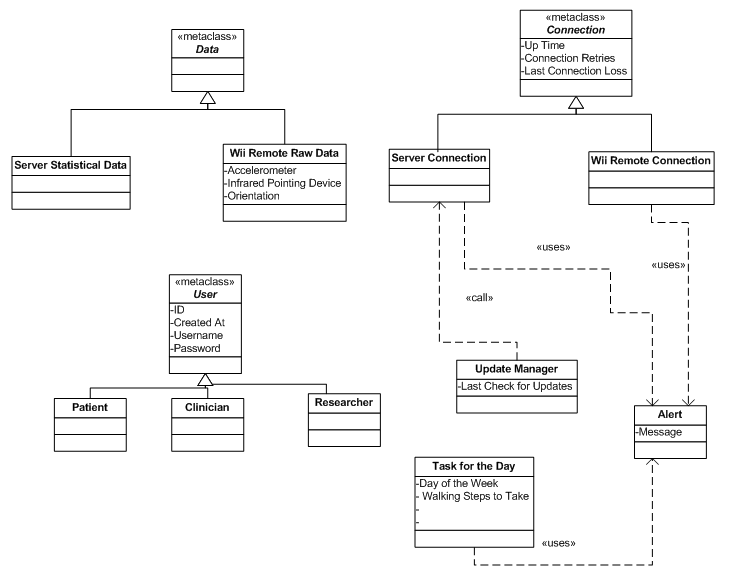
\includegraphics[width=6in,height=4.82in]{objstuff.png}
\caption{Preliminary object orient domain analysis for the server and pda software.}
\label{fig: prelim ooda}
\end{figure}

\begin{enumerate}
\item User - Abstract base class that represents all users of the system. This class will provide information pertaining to when the user was created, username/password, and ID. 
\item Patient - The Patient user class must be appropriately implemented to model user interaction with the Wii Remote and PDA.
\item Clinician - The Clinician domain object must be modeled to allow for logins/interaction with the Web UI.  
\item Researcher - The Researcher domain object must be modeled to allow for logins/interaction with the Web UI. 
\item Connection - This object is the base class for all connections made by the PDA. It will contain information regarding up time, number of connection retries, and last lost connection.
\item Server Connection - This object will manage the connection between the PDA and the Server. This includes initial connection set-up, as well as connection retries when the connection is lost. 
\item Wii Remote-PDA Connection - This object will manage the connection between the Wii Remote and the PDA. This includes information pertaining to which Patient the pair of devices is assigned to.
\item Update Manager - This object will deal with retrieving task updates as well as data dumping to the Server. The Update Manager will use the Server Connection object to establish a connection between the PDA and Server.
\item Alert - This object will display alert messages on the PDA. This will be used for connection messages, task updates, exercise alerts, etc.   
\item Data - This object will represent all of the exercise data that is collected and analyzed. This includes the raw data that is gathered from the Wii Remote, as well as computed statistics, graphs, charts, etc. 
\item Wii Remote Exercise Raw Data - This object will inherit from Data and will represent all of the raw exercise data that is gathered from the Wii Remote over bluetooth. The data represented in this object will be run through algorithms to compute relevant real-time statistics on the PDA. 
\item Server Statistical Data - This object will represent all of the statistics computed on the Server. This includes information pertaining to Patient Health Charts, Daily Task PDA Statistics, Group Patient Charts, and Patient Completion Charts.  
\item Task for the Day - This object will represent the number of walking steps a Patient must achieve in a given day. 
\end{enumerate}

\section{Operational Scenarios}
\begin{enumerate}
\item The PDA and the Wii Remote must be connected before they are given to a Patient.  An alert is sent to the PDA when it receives connection from the Wii Remote and sends an acknowledgement.  If the PDA and Wii Remote are not paired, they must have a discoverable mode for a connection to occur in the future.  The PDA must also have a connection with the server to send data to be stored in a database.

\item The PDA receives data from the Wii Remote and it is stored in the PDA memory.  The PDA will notify the Patient of PDA Statistics in real time.  The PDA starts running scripts for analysis of stored data.  The PDA dumps data to the server. The PDA connects to the server and sends the username and password. The server reponds with an authentication complete if the username and password are correct.  If the connection fails the PDA keeps trying to reconnect and dump data to the server.

\item There must be a web UI hosted by a server that provides a way for all users to access data available to them.  Each user will have a unique username and password.

\item The user starts the application on the PDA by entering a username and password and is directed to their account page with the PDA Statistics Page displayed.  The PDA will connect to the server to itemize the Patient's tasks for the day in an easy to read font.  The tasks page will also have a close button to return the user to the home page.  The PDA will display an alert message for the Patient when a task is complete.

\item The Clinician will log into the web UI by entering a username and password.  The Clinician will have the ability to create a profile for a new Patient with all data being hosted on a database, this profile will be linked to a specified PDA and Wii Remote.  The Clinician will also be able to graph Patient data.  Data should be in human readable form.

\item The Clinician can also view various reports and graphs on a certain Patient's progress.  Also on the web UI will be a Patient Health Chart displaying how the Patient has improved or worsened over time.  The web UI will display a list of Patients for the Clinician currently logged in.  The server should provide links to each Patient's profile for the Clinician to view.  The web UI should also provide the Clinician the ability to change or modify tasks for Patients.

\item The Researcher will log into the web UI by entering a username and password.

\item The PDA will monitor the status of the Wii Remote battery.  When the battery power is low, the PDA will alert the user by displaying a message and causing the Wii Remote to vibrate.
\end{enumerate}



\section{Overall Test Plan}
\subsection{Web UI Testing}
\subsubsection{Clinician Access}
\begin{enumerate}
\item The tester has a Clinician account on the server and logs into the Web UI.
\item The tester sees the main splash screen with the available links including: Patient List, Add New Patient, and Remove Patient.
\item Click the Add New Patient link.
\item The add new Patient form is displayed which requires the Clinician to enter the profile information and current task for the Patient.
\item Enter the profile information and click save.
\item The information is saved to the database and the Clinician is returned to the main splash screen.
\item Next, click the Patient List link. The Patient listing which includes any previously added Patients and the newly added Patient is displayed.
\item Click the newly added Patient name. The Patient's profile is displayed along with the option to change the Patient's task.
\item Click the link to change the Patient's task. The change Patient task page is displayed with the current task in an editable format.
\item The task is changed and the page is submitted. The new task is saved to the database and the Patient's profile page is redisplayed.
\item Log out of the Clinician's account.
\end{enumerate}
\subsubsection{Researcher Access}
\begin{enumerate}
\item The tester has a Researcher account ont he server and logs into the Web UI.
\item The main splash screen is displayed with links including: View Patient Groups, View Single Patient.
\item Click the View Patient Groups link. The listing of Patient groups is displayed.
\item Click a group of Patients. The graphs and charts displaying the aggregate data for this group of Patients are displayed.
\item Return to the main splash screen using the Home link. The splash screen is displayed.
\item Click the view single Patient link. A list of Patient numbers is displayed.
\item Click a Patient number. A profile for the Patient should appear, but the page should not contain any personal information for the Patient except for age, sex and medical conditions. The page should not display a Patient's name, address, or exact birthday. 
\item The page should also display a series of graphs which represents the Patient's progress and completion of each task for each day.
\item Log out of the Researcher's account.
\end{enumerate}

\subsection{PDA Testing}
\subsubsection{Setup Device}
\begin{enumerate}
\item The tester turns on the PDA and enters the Activity Monitor application.
\item The main application screen appears. The tester enters the setup mode, as a Clinician would.
\item In setup mode, the device displays edit fields to enter the necessary information to connect to the Server. This includes the Patient's client id and a password.
\item The tester saves the setup information for connecting to the Server by clicking Next. The screen for pairing with the Wii Remote is displayed.
\item The tester initiates a Bluetooth search for the Wii Remote and once found by the PDA, pairs the PDA and the Wii Remote.
\item Click next. The main splash screen is again displayed with a message box indicating the settings were saved and the device is now ready.
\item The tester turns the device off and back on by pressing the off button. When the device starts backup, the main splash screen of the application is the first thing observed.
\end{enumerate}
\subsubsection{Patient Activities}
\begin{enumerate}
\item The PDA is setup and can establish a connection to the server.
\item From the main splash screen on the PDA click the Daily Task button.
\item The daily task as recored in the database is displayed in a large easy to read font on the PDA.  The task is not marked completed.
\item Click the back button. The main splash screen is displayed.
\item As the tester walks with the PDA and Wii Remote, the stats on the splash screen are updated. This includes the number of steps taken and the current step/minute walking rate.
\item The tester walks far enough or fast enough to complete the task. When the task is completed the Wii Remote vibrates and makes a noise. The PDA displays a message indicating the task for the day was completed.
\item The tester continues walking and the main splash screen continues to update.
\item Click the Dialy Task button. The task for the day is displayed and marked completed.
\item Click the back button. The main splash screen is displayed.
\item The tester changes the task on the server and waits until the PDA updates the task for the next day.
\item At 11:59PM click the Daily Task button. The old task is still displayed. Click back and the main splash screen is displayed.
\item At 12:01AM click the Daily Task button. The new task as updated the day before is displayed.  Click the back button and the main splash screen is displayed.
\end{enumerate}
\subsubsection{Dump Data to Server}
\begin{enumerate}
\item The tester has completed the daily task for the previous day and the periodic data dump to server is about to occur between the PDA and the server.
\item There is no noticible difference in the operation of the smart pedometer system as the data dump occurs.
\item The tester logs into the Web UI as the Clinician and checks to be sure the data for yesterday appears in the graphs and charts for the Patient.
\item The next day the tester disables the server and again waits for the data dump to occur.
\item The PDA attempts to dump the data, but cannot find the server. After several attempts which are apparent to the Patient, a message appears on the PDA.
\item When the Patient picks up the Wii Remote and begins to walk, the Wii Remote vibrates and makes a noise indicating there is a message on the PDA.
\item Click OK on the message. The message disappears and the application behaves normally.
\end{enumerate}

\end{document}

